% Proposta de figura para a seção "Integração entre ARIMA e GARCH" do Cap. I
% (12/11/2026, pedido do autor). NÃO é parte do TG: o autor quer analisar antes
% de decidir. Figuras em fig-integracao-a.tex a -h.tex (12/11), compiladas
% pelo Makefile desta pasta.
\documentclass[11pt,a4paper]{article}
\usepackage[T1]{fontenc}
\usepackage[brazilian]{babel}
\usepackage{mathptmx}
\usepackage[a4paper,margin=2.4cm]{geometry}
\usepackage{graphicx}
\usepackage[font=small,labelfont=bf]{caption}
\usepackage[most]{tcolorbox}
\usepackage[hidelinks]{hyperref}
\setlength{\parskip}{0.45em}
\setlength{\parindent}{0pt}

\definecolor{cesc}{RGB}{220,50,32}
\definecolor{cmod}{RGB}{0,90,181}
\newtcolorbox{ideia}[1][]{colback=cmod!5, colframe=cmod!70, fonttitle=\bfseries, title={#1}, arc=2pt, boxrule=0.6pt}
\newtcolorbox{cuidado}[1][]{colback=cesc!4, colframe=cesc!70, fonttitle=\bfseries, title={#1}, arc=2pt, boxrule=0.6pt}

\title{Figura proposta para o Capítulo I\\[2pt]\large o ARIMA e o GARCH integrados}
\author{Material de análise, fora do TG}
\date{12 de novembro de 2026}

\begin{document}
\maketitle

O Capítulo~I apresenta o ARIMA com a Figura~5 (as etapas de aplicação do modelo) e
o GARCH com a Figura~6 (como a volatilidade prevista é formada). A seção
``Integração entre ARIMA e GARCH'' explica em palavras como os dois trabalham
juntos, mas não tem figura. Este relatório traz oito propostas para ela, e a ideia é
escolher uma só.

As propostas A, B e C partem de onde a Figura~5 termina. As saídas dela, ``Sinal da previsão:
direção da operação'' e ``Resíduos: real menos previsto'', aparecem aqui com as
mesmas palavras e o mesmo formato, para o leitor reconhecer a ligação. O estilo
(caixas cinza, trapézios para dados, fonte) é o mesmo das Figuras~5 e~6.

\section{Proposta A: as duas perguntas}

\begin{figure}[h]
\centering
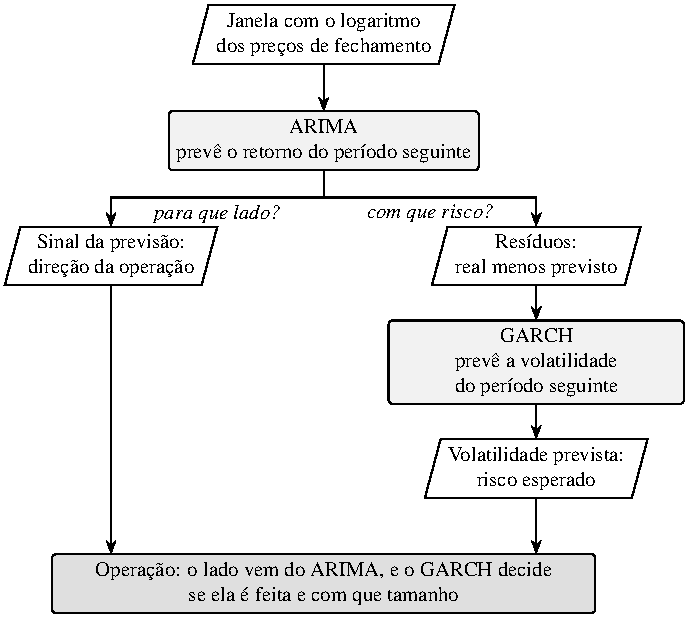
\includegraphics{fig-integracao-a.pdf}
\caption{Proposta A (título no TG: ``Integração entre ARIMA e GARCH'')}
\end{figure}

O ARIMA recebe a janela de preços e faz a previsão. Dela saem dois caminhos. O da
esquerda é o sinal da previsão, que diz para que lado operar. O da direita são os
resíduos, que o GARCH usa para prever a volatilidade, ou seja, o risco. Os dois se
encontram na operação: o lado vem do ARIMA, e o GARCH decide se ela é feita e com
que tamanho. As duas perguntas em itálico, logo abaixo da bifurcação, são as do
segundo parágrafo da seção (``essa combinação permite separar duas perguntas'').

O desenho mostra também a regra que o trabalho repete várias vezes: o GARCH não
tem seta para a direção. O único caminho até o lado da operação passa pelo ARIMA.

Onde entraria: no fim do segundo parágrafo da seção, antes da subseção ``Uso da
volatilidade prevista na operação''. Frase sugerida para chamá-la: ``A Figura~X
resume essa divisão de papéis.''

\clearpage
\section{Proposta B: com o filtro e o ajuste da posição}

\begin{figure}[h]
\centering
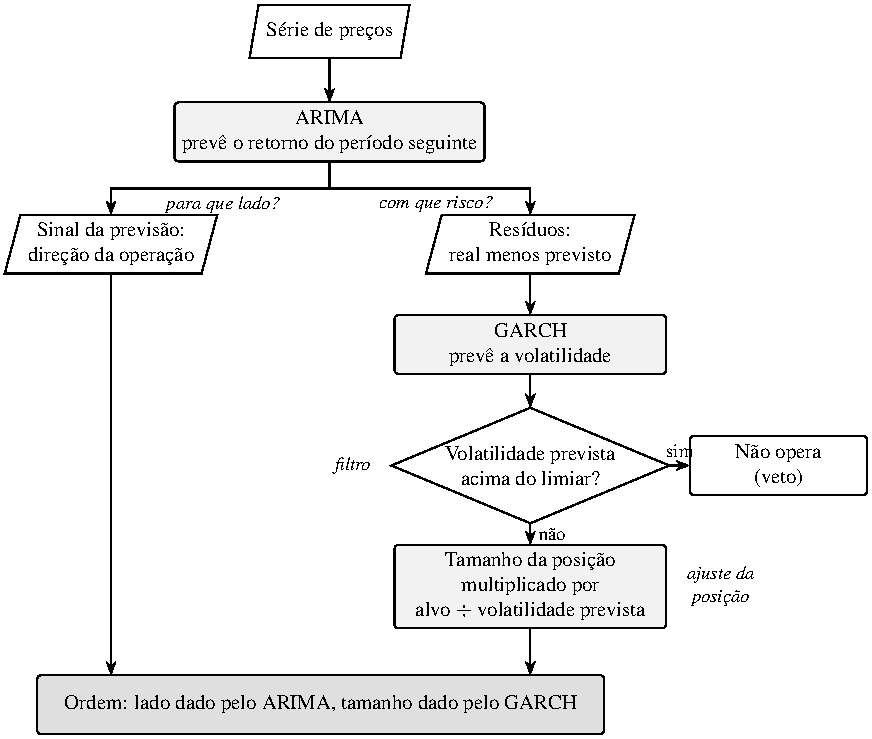
\includegraphics{fig-integracao-b.pdf}
\caption{Proposta B, revista em 12/11/2026}
\end{figure}

É a proposta A com o lado do GARCH aberto nas duas maneiras de usar a volatilidade
prevista. Primeiro o filtro compara a volatilidade prevista com o limiar e, se ela
estiver acima, a operação é vetada. Se não estiver, o ajuste da posição multiplica
o tamanho pela razão entre o alvo e a volatilidade prevista. A ordem sai com o lado
do ARIMA e o tamanho do GARCH. Na revisão de 12/11, a entrada passou a ser ``Série
de preços'', e as duas perguntas da proposta A foram acrescentadas logo abaixo da
bifurcação.

Ela tem um problema de leitura, apontado pelo autor. A seta do sinal da previsão
desce direto até a ordem, sem passar pelo filtro, e dá a impressão de que o sinal
sempre chega lá, mesmo quando a operação é vetada. A proposta C corrige isso.

\clearpage
\section{Proposta C: o sinal só segue se não houver veto}

\begin{figure}[h]
\centering
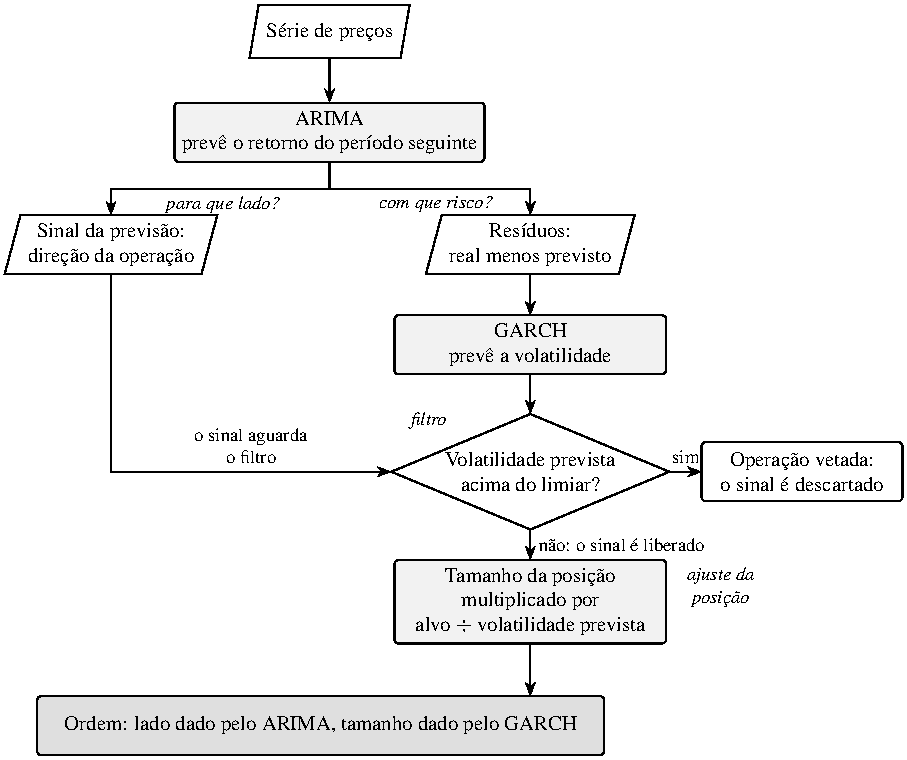
\includegraphics{fig-integracao-c.pdf}
\caption{Proposta C (título no TG: ``Integração entre ARIMA e GARCH na operação'')}
\end{figure}

A diferença para a B está no caminho do sinal. Em vez de descer direto até a
ordem, a seta do sinal da previsão entra no filtro, junto com a volatilidade
prevista pelo GARCH. O filtro passa a ser o ponto em que os dois caminhos se
encontram, e a pergunta dele decide o destino do sinal. Se a volatilidade prevista
estiver acima do limiar, a operação é vetada e o sinal é descartado. Se não
estiver, o sinal é liberado, o ajuste da posição define o tamanho, e a ordem sai
com o lado do ARIMA e o tamanho do GARCH.

Assim o desenho mostra, sem precisar de texto, as duas regras da integração. A
primeira é que só o ARIMA dá a direção, porque o único caminho até o lado da ordem
começa no sinal da previsão. A segunda é que o GARCH tem a palavra final sobre se a
operação acontece, porque o sinal só passa pelo filtro quando não há veto.

Onde entraria: no fim da subseção ``Uso da volatilidade prevista na operação'',
depois do parágrafo ``As duas maneiras podem ser combinadas'', que é o que o
desenho mostra. Frase sugerida: ``A Figura~X mostra o caminho completo, com as
duas maneiras combinadas.''

\section{Proposta D: mais simples, com um caminho só}

\begin{figure}[h]
\centering
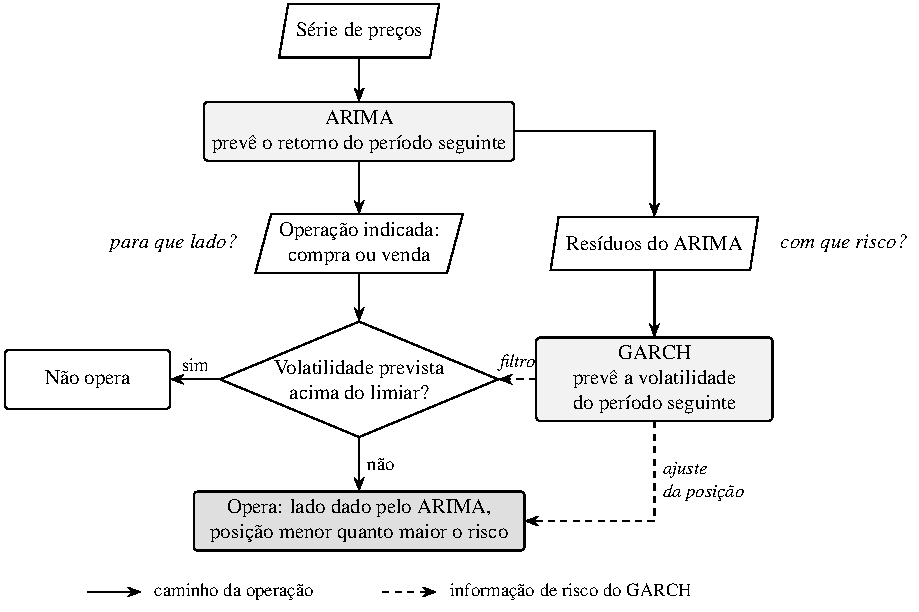
\includegraphics{fig-integracao-d.pdf}
\caption{Proposta D (mesmo título no TG: ``Integração entre ARIMA e GARCH na operação'')}
\end{figure}

\textbf{A C está correta?} No conteúdo, sim: só o ARIMA dá o lado, o GARCH decide
se a operação é feita e de que tamanho, e é isso que o robô faz. O problema está
na forma. Um losango é uma pergunta, e numa figura desse tipo só deve entrar nele
o que está sendo decidido. Na C entram duas setas, a do sinal e a da
volatilidade, e o leitor pode entender que o filtro compara uma com a outra, ou
que a direção participa da decisão de vetar. Não participa: o filtro olha só a
volatilidade prevista. Além disso, a C tem a fórmula do ajuste (o tamanho
multiplicado pela razão entre volatilidades), que é detalhe do Capítulo~II.

\textbf{O que muda na D.} A figura passa a ter um caminho principal só, de cima
para baixo, com setas cheias: a série de preços, o ARIMA, a operação indicada
(compra ou venda), a pergunta do filtro e o resultado. Esse é o caminho da
operação, e é ele que entra no losango. O GARCH fica ao lado, alimentado pelos
resíduos do ARIMA, e entra só com setas tracejadas, que são informação, não
caminho. Uma vai para o filtro, que usa a volatilidade prevista para responder à
pergunta. A outra vai para a caixa final, que usa a mesma volatilidade para
definir o tamanho da posição. A legenda embaixo diz o que é cada tipo de seta.

O resto foi simplificado. A fórmula saiu e no lugar dela ficou a frase ``posição
menor quanto maior o risco'', que é o que o Capítulo~I diz do ajuste da posição.
O veto virou ``Não opera'', e a liberação virou a própria caixa ``Opera'', que
lembra que o lado vem do ARIMA. As perguntas ``para que lado?'' e ``com que
risco?'' continuam, uma ao lado de cada modelo.

\textbf{Como se lê, em uma frase.} O ARIMA diz para que lado operar, o GARCH diz
com que risco, e a operação só é feita quando o risco previsto não passa do
limiar, com uma posição menor quanto maior esse risco.

\textbf{Se entrar no TG.} Substitui a figura atual (a C) no mesmo lugar, sem
mudar o título. A frase que chama a figura no Capítulo~I continua valendo. Só
um ajuste de palavra seria bom, porque a D fala em ``operação indicada'', e não em
``sinal'' e ``ordem''. Sugestão: ``A operação indicada pelo ARIMA só é feita quando
o filtro não a veta, e o tamanho da posição é ajustado pela volatilidade prevista
pelo GARCH.'' A D é cerca de 2,5 cm mais
baixa que a C (294 contra 365 pontos de altura), o que muda um pouco a paginação
do Capítulo~I. Isso só se confirma compilando, e aí se confere de novo se alguma
ilustração corta parágrafo.

\section{Proposta E: no molde da figura do PTG}

\begin{figure}[h]
\centering
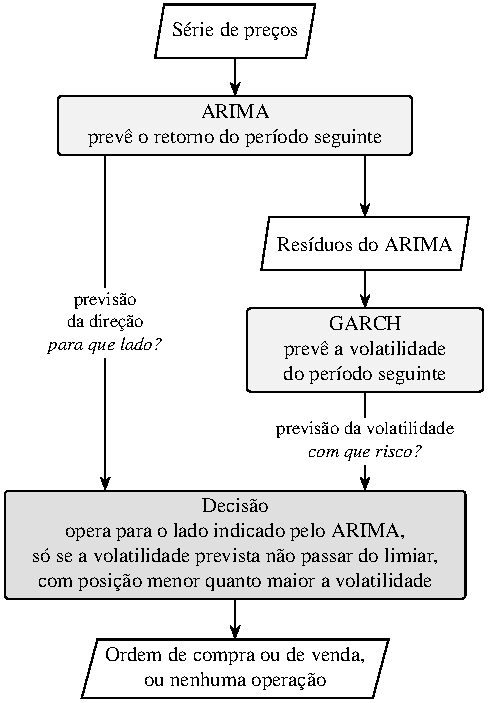
\includegraphics{fig-integracao-e.pdf}
\caption{Proposta E (mesmo título no TG: ``Integração entre ARIMA e GARCH na operação'')}
\end{figure}

A D ainda precisava de legenda para separar seta cheia de seta tracejada, o que
mostra que ela não se explica sozinha. A E segue o molde da figura ``Modelo
Completo'' do PTG (cópia em \texttt{ia/rascunhos/figuras\_ptg\_removidas/}), sem
o que saiu do escopo (LSTM e indicadores). Naquela figura cada seta diz o que
carrega, e os ramos se juntam numa caixa de decisão. Aqui é igual. A série de
preços entra no ARIMA, que se divide em dois ramos. À esquerda desce a previsão da
direção, com a pergunta ``para que lado?''. À direita, os resíduos vão para o
GARCH, e dele desce a previsão da volatilidade, com a pergunta ``com que risco?''.
Os dois ramos chegam juntos à caixa ``Decisão'', que diz em três linhas a regra
inteira (o lado vem do ARIMA, só se opera abaixo do limiar, e a posição é menor
quanto maior a volatilidade). Embaixo sai a ordem, ou nenhuma operação.

Não há losango, legenda, fórmula nem tipos diferentes de seta. Toda seta é do
mesmo tipo e tem o nome do que leva. A condição que a C mostrava com o losango
(o sinal só segue se não houver veto) agora está escrita na caixa da decisão
(``só se a volatilidade prevista não passar do limiar'') e na saída (``ou nenhuma
operação'').

\textbf{Se entrar no TG.} Substitui a figura atual (a C) no mesmo lugar, com o
mesmo título. A frase do Capítulo~I que chama a figura continua valendo como está.
A E é mais estreita e um pouco mais baixa que a C (338 contra 365 pontos de
altura), e depois de compilar se confere de novo se alguma ilustração corta
parágrafo.

\section{Proposta F: o meio-termo entre a C e a E}

\begin{figure}[h]
\centering
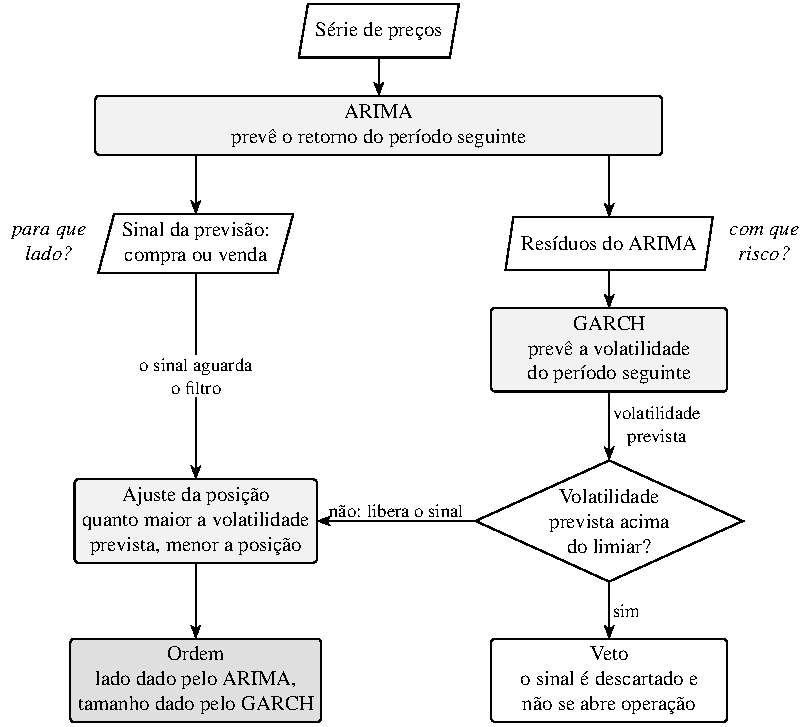
\includegraphics{fig-integracao-f.pdf}
\caption{Proposta F (mesmo título no TG: ``Integração entre ARIMA e GARCH na operação'')}
\end{figure}

A E se lê sozinha, mas junta tudo numa caixa de texto e esconde as etapas. A F
mantém o que a E tem de claro (setas com o nome do que levam, sem legenda e sem
fórmula) e traz de volta as etapas da C: o filtro como pergunta, o veto e o
ajuste da posição.

A diferença para a C está no lugar do losango. Ele agora fica no ramo do GARCH, e
só a volatilidade prevista entra nele, porque o filtro só olha a volatilidade. O
sinal do ARIMA não passa pelo losango: desce pelo seu próprio ramo até o ajuste da
posição e espera lá (``o sinal aguarda o filtro''). Se a volatilidade prevista
estiver acima do limiar, a saída é o veto, à direita. Se não estiver, o filtro
libera o sinal, a posição é ajustada e sai a ordem, à esquerda, com o lado do
ARIMA e o tamanho do GARCH.

Assim a figura termina com os dois resultados possíveis lado a lado, a ordem e o
veto, e cada ramo continua respondendo à sua pergunta, ``para que lado?'' à
esquerda e ``com que risco?'' à direita.

\textbf{Se entrar no TG.} Substitui a figura atual (a C) no mesmo lugar, com o
mesmo título. A frase do Capítulo~I que chama a figura continua valendo como está
(``O sinal da previsão do ARIMA só chega à ordem quando o filtro não veta a
operação\ldots''), e as palavras dela agora aparecem na própria figura. A F tem
349 pontos de altura, contra 365 da C, e depois de compilar se confere de novo se
alguma ilustração corta parágrafo.

\section{Proposta G: a B com as duas faixas}

\begin{figure}[h]
\centering
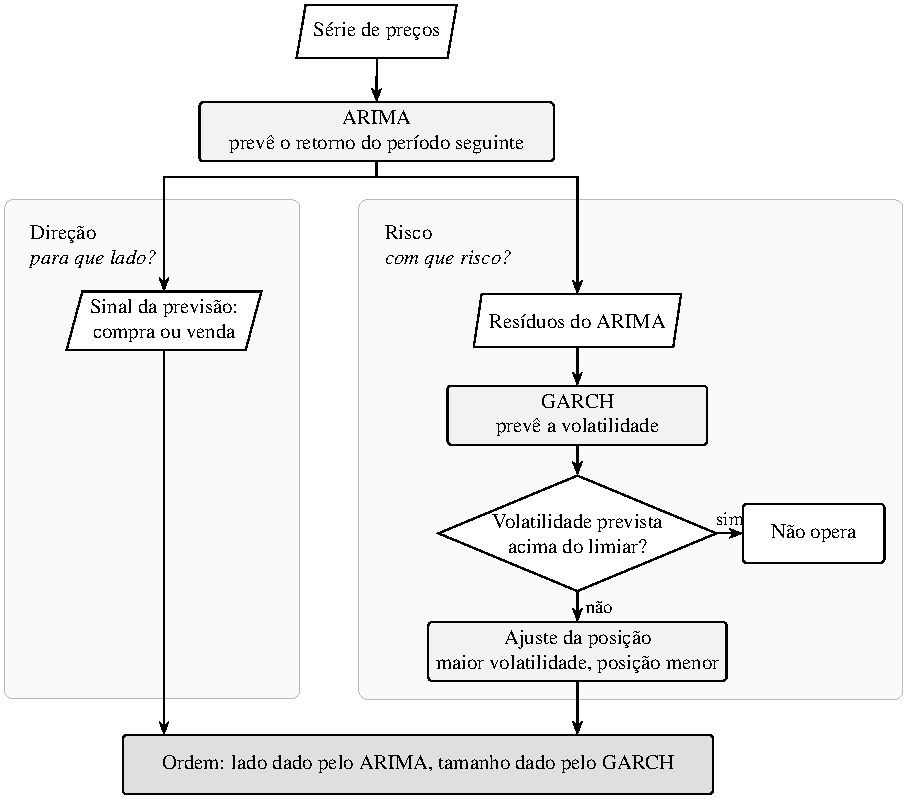
\includegraphics{fig-integracao-g.pdf}
\caption{Proposta G (mesmo título no TG: ``Integração entre ARIMA e GARCH na operação'')}
\end{figure}

O autor achou a B a melhor das seis, mas ainda complexa. A G é a B com três
mudanças. A primeira é que cada ramo ficou dentro de uma faixa com nome, Direção
(\textit{para que lado?}) e Risco (\textit{com que risco?}). A integração dos dois
modelos aparece no próprio desenho: as duas faixas nascem do mesmo ARIMA e só se
juntam embaixo, na ordem, que recebe o lado de uma e o tamanho da outra. A
segunda é que a fórmula do ajuste saiu, e a caixa diz só ``maior volatilidade,
posição menor''. A terceira é que os textos ficaram mais curtos (``Não opera'' em
vez de ``Não opera (veto)'', ``Resíduos do ARIMA'' em vez de ``Resíduos: real menos
previsto'') e os rótulos soltos ``filtro'' e ``ajuste da posição'' saíram, porque o
losango e a caixa já dizem o que fazem.

O losango continua onde estava na B, na faixa do risco, e recebe só a volatilidade
prevista, que é o que o filtro olha. A direção não passa por ele.

\textbf{Se entrar no TG.} Substitui a figura atual (a C) no mesmo lugar, com o
mesmo título. A frase do Capítulo~I que chama a figura continua valendo como está.
A G tem 384 pontos de altura, contra 365 da C, e depois de compilar se confere de
novo se alguma ilustração corta parágrafo.

\section{Proposta H: a G sem as faixas, mais espaçada}

\begin{figure}[h]
\centering
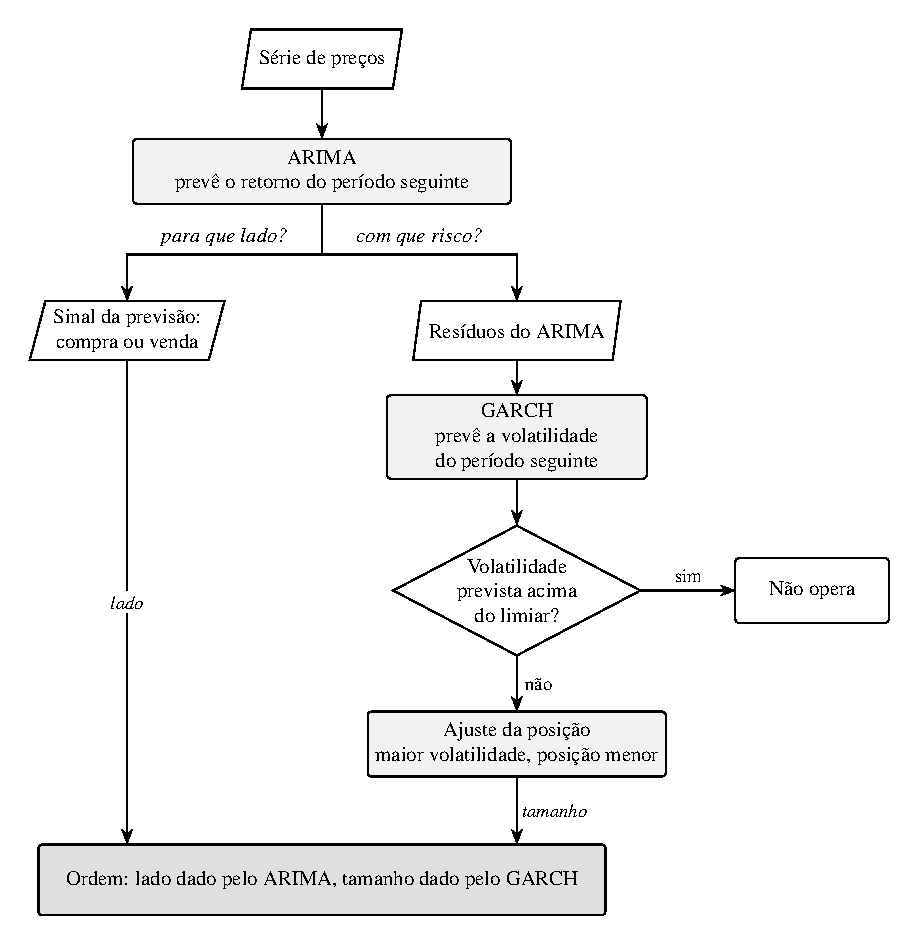
\includegraphics[width=0.85\textwidth]{fig-integracao-h.pdf}
\caption{Proposta H (mesmo título no TG: ``Integração entre ARIMA e GARCH na operação'')}
\end{figure}

A pedido do autor, as faixas da G saíram. As perguntas voltaram para cima da
divisão dos ramos, como na B. A seta do ``sim'' até ``Não opera'' ficou mais longa,
e todas as caixas ganharam mais espaço entre si. As duas setas que chegam à ordem
agora têm nome, ``lado'' e ``tamanho'', e isso mostra a integração no próprio
desenho: a ordem recebe o lado do ARIMA e o tamanho do GARCH. O arquivo tem margem
branca e também existe em PNG (\texttt{fig-integracao-h.png}, 300~dpi), para ser
copiado.

\section{Qual escolher}

\begin{ideia}[Recomendação: a proposta H]
A H é a B que o autor preferiu, sem fórmula, sem rótulos soltos e com mais
espaço. Os dois ramos saem do mesmo ARIMA e se juntam na ordem, com as setas
``lado'' e ``tamanho'' dizendo o que cada um entrega.
\end{ideia}

\begin{cuidado}[Diferença de palavras em relação à Figura~5]
A D e a E não repetem as palavras da saída da Figura~5 (``Sinal da previsão: direção da
operação'' e ``Resíduos: real menos previsto''). A D usa ``Operação indicada: compra
ou venda'', a E usa ``previsão da direção'', e as duas usam ``Resíduos do
ARIMA''. São mais curtas. O sentido é o mesmo. Se
quiser a ligação literal entre as figuras, dá para trocar só esses dois textos.
\end{cuidado}

\begin{cuidado}[O que as propostas C a H simplificam]
O desenho mostra o filtro e o ajuste sempre juntos. No robô, cada um também foi
testado sozinho. O veto descarta o sinal, ou seja, a operação nova não é feita,
mas a posição que já estava aberta pode ser mantida ou encerrada, conforme a
configuração. O ajuste também tem limites (um quarto e o dobro do tamanho normal).
Tudo isso é do Capítulo~II e não cabe no Capítulo~I. Se a banca perguntar o que
acontece com a posição aberta no dia do veto, a resposta está na subseção ``Uso do
GARCH na decisão'' do Capítulo~II.
\end{cuidado}

\begin{cuidado}[A entrada]
A entrada das propostas B e C agora é ``Série de preços''. A Figura~5 usa ``Janela
com o logaritmo dos preços de fechamento''. A diferença não chega a ser um erro,
porque esta figura mostra a ideia, e a Figura~5, as etapas. Se quiser as duas
iguais, dá para trocar a entrada da Figura~5 também. O uso do logaritmo está
explicado no Capítulo~II, em ``Preparação dos preços''.
\end{cuidado}

\end{document}
